\documentclass[11pt, a4paper]{article}

% --- Packages ---
\usepackage[margin=1in]{geometry}    % Standard 1-inch margins
\usepackage{amsmath, amssymb}        % Math typesetting
\usepackage{graphicx}                % Image handling
\usepackage{hyperref}                % Clickable links
\usepackage{xcolor}                  % Color support
\usepackage{booktabs}                % Professional tables
\usepackage{cite}                    % Citation management
\usepackage{minted}
\usepackage{listings}
\usepackage{booktabs}
\usepackage{float}
% --- Link Setup ---
\hypersetup{
    colorlinks=true,
    linkcolor=blue,
    filecolor=magenta,
    urlcolor=cyan,
    citecolor=blue,
}

% --- Title Information ---
\title{\textbf{Project 2 Report}\\ \large INFSCI 2591 - Algorithm Design}
\author{Abhay Kumara Sri Krishna Nandiraju \\ University of Pittsburgh}
\date{Spring 2026}

\begin{document}

\maketitle

% \begin{abstract}
% This is a brief summary of your project. State the problem you are solving, the methodology or architecture you used, and the primary results or performance metrics you achieved. Keep it concise, usually around 150-200 words.
% \end{abstract}

% --- Main Content ---
\section{Test Case Results}

\subsection{Dijkstra Algorithm using 2D Array}

\begin{table}[h!] % [H] forces the table to stay exactly HERE
\centering
\begin{tabular}{|l|l|l|p{8cm}|} % p{8cm} forces the Path column to wrap
\hline
\textbf{Test Case} & \textbf{Route} & \textbf{Distance (ft)} & \textbf{Path} \\ \hline
1 & 192 $\rightarrow$ 163 & 819 & [192, 157, 194, 158, 161, 163] \\ \hline
2 & 138 $\rightarrow$ 66 & 2728 & [138, 162, 136, 159, 119, 116, 114, 112, 70, 110, 79, 108, 107, 103, 105, 85, 67, 66] \\ \hline
3 & 465 $\rightarrow$ 22 & 6738 & [465, 377, 380, 372, 363, 364, 305, 247, 210, 233, 201, 170, 128, 98, 78, 41, 23, 22] \\ \hline
\end{tabular}
\caption{Test Case results using Dijkstra's algorithm with 2D-array}
\label{dij2d}
\end{table}


\subsection{Dijkstra Algorithm using Linked List}

\begin{table}[h!] % [H] forces the table to stay exactly HERE
\centering
\begin{tabular}{|l|l|l|p{8cm}|} % p{8cm} forces the Path column to wrap
\hline
\textbf{Test Case} & \textbf{Route} & \textbf{Distance (ft)} & \textbf{Path} \\ \hline
1 & 192 $\rightarrow$ 163 & 819 & [192, 157, 194, 158, 161, 163] \\ \hline
2 & 138 $\rightarrow$ 66 & 2728 & [138, 162, 136, 159, 119, 116, 114, 112, 70, 110, 79, 108, 107, 103, 105, 85, 67, 66] \\ \hline
3 & 465 $\rightarrow$ 22 & 6738 & [465, 377, 380, 372, 363, 364, 305, 247, 210, 233, 201, 170, 128, 98, 78, 41, 23, 22] \\ \hline
\end{tabular}
\caption{Test Case results using Dijkstra's algorithm with Linked List}
\label{dijll}
\end{table}

\subsection{Floyd Algorithm using 2D Array}

\begin{table}[h!] % [H] forces the table to stay exactly HERE
\centering
\begin{tabular}{|l|l|l|p{8cm}|} % p{8cm} forces the Path column to wrap
\hline
\textbf{Test Case} & \textbf{Route} & \textbf{Distance (ft)} & \textbf{Path} \\ \hline
1 & 192 $\rightarrow$ 163 & 819 & [192, 157, 194, 158, 161, 163] \\ \hline
2 & 138 $\rightarrow$ 66 & 2728 & [138, 162, 136, 159, 119, 116, 114, 112, 70, 110, 79, 108, 107, 103, 105, 85, 67, 66] \\ \hline
3 & 465 $\rightarrow$ 22 & 6738 & [465, 377, 380, 372, 363, 364, 305, 247, 210, 233, 201, 170, 128, 98, 78, 41, 23, 22] \\ \hline
\end{tabular}
\caption{Test Case results using Floyd's algorithm with 2D Array}
\label{floyd2d}
\end{table}


\subsection{Floyd Algorithm using Linked List}

\begin{table}[h!] % [H] forces the table to stay exactly HERE
\centering
\begin{tabular}{|l|l|l|p{8cm}|} % p{8cm} forces the Path column to wrap
\hline
\textbf{Test Case} & \textbf{Route} & \textbf{Distance (ft)} & \textbf{Path} \\ \hline
1 & 192 $\rightarrow$ 163 & 819 & [192, 157, 194, 158, 161, 163] \\ \hline
2 & 138 $\rightarrow$ 66 & 2728 & [138, 162, 136, 159, 119, 116, 114, 112, 70, 110, 79, 108, 107, 103, 105, 85, 67, 66] \\ \hline
3 & 465 $\rightarrow$ 22 & 6738 & [465, 377, 380, 372, 363, 364, 305, 247, 210, 233, 201, 170, 128, 98, 78, 41, 23, 22] \\ \hline
\end{tabular}
\caption{Test Case results using Floyd's algorithm with Linked List}
\label{floydll}
\end{table}

\vspace{-3mm}

\section{Time Performance Plots}
\subsection{Dijkstra's Algorithm}
\begin{figure}[H]
    \centering
    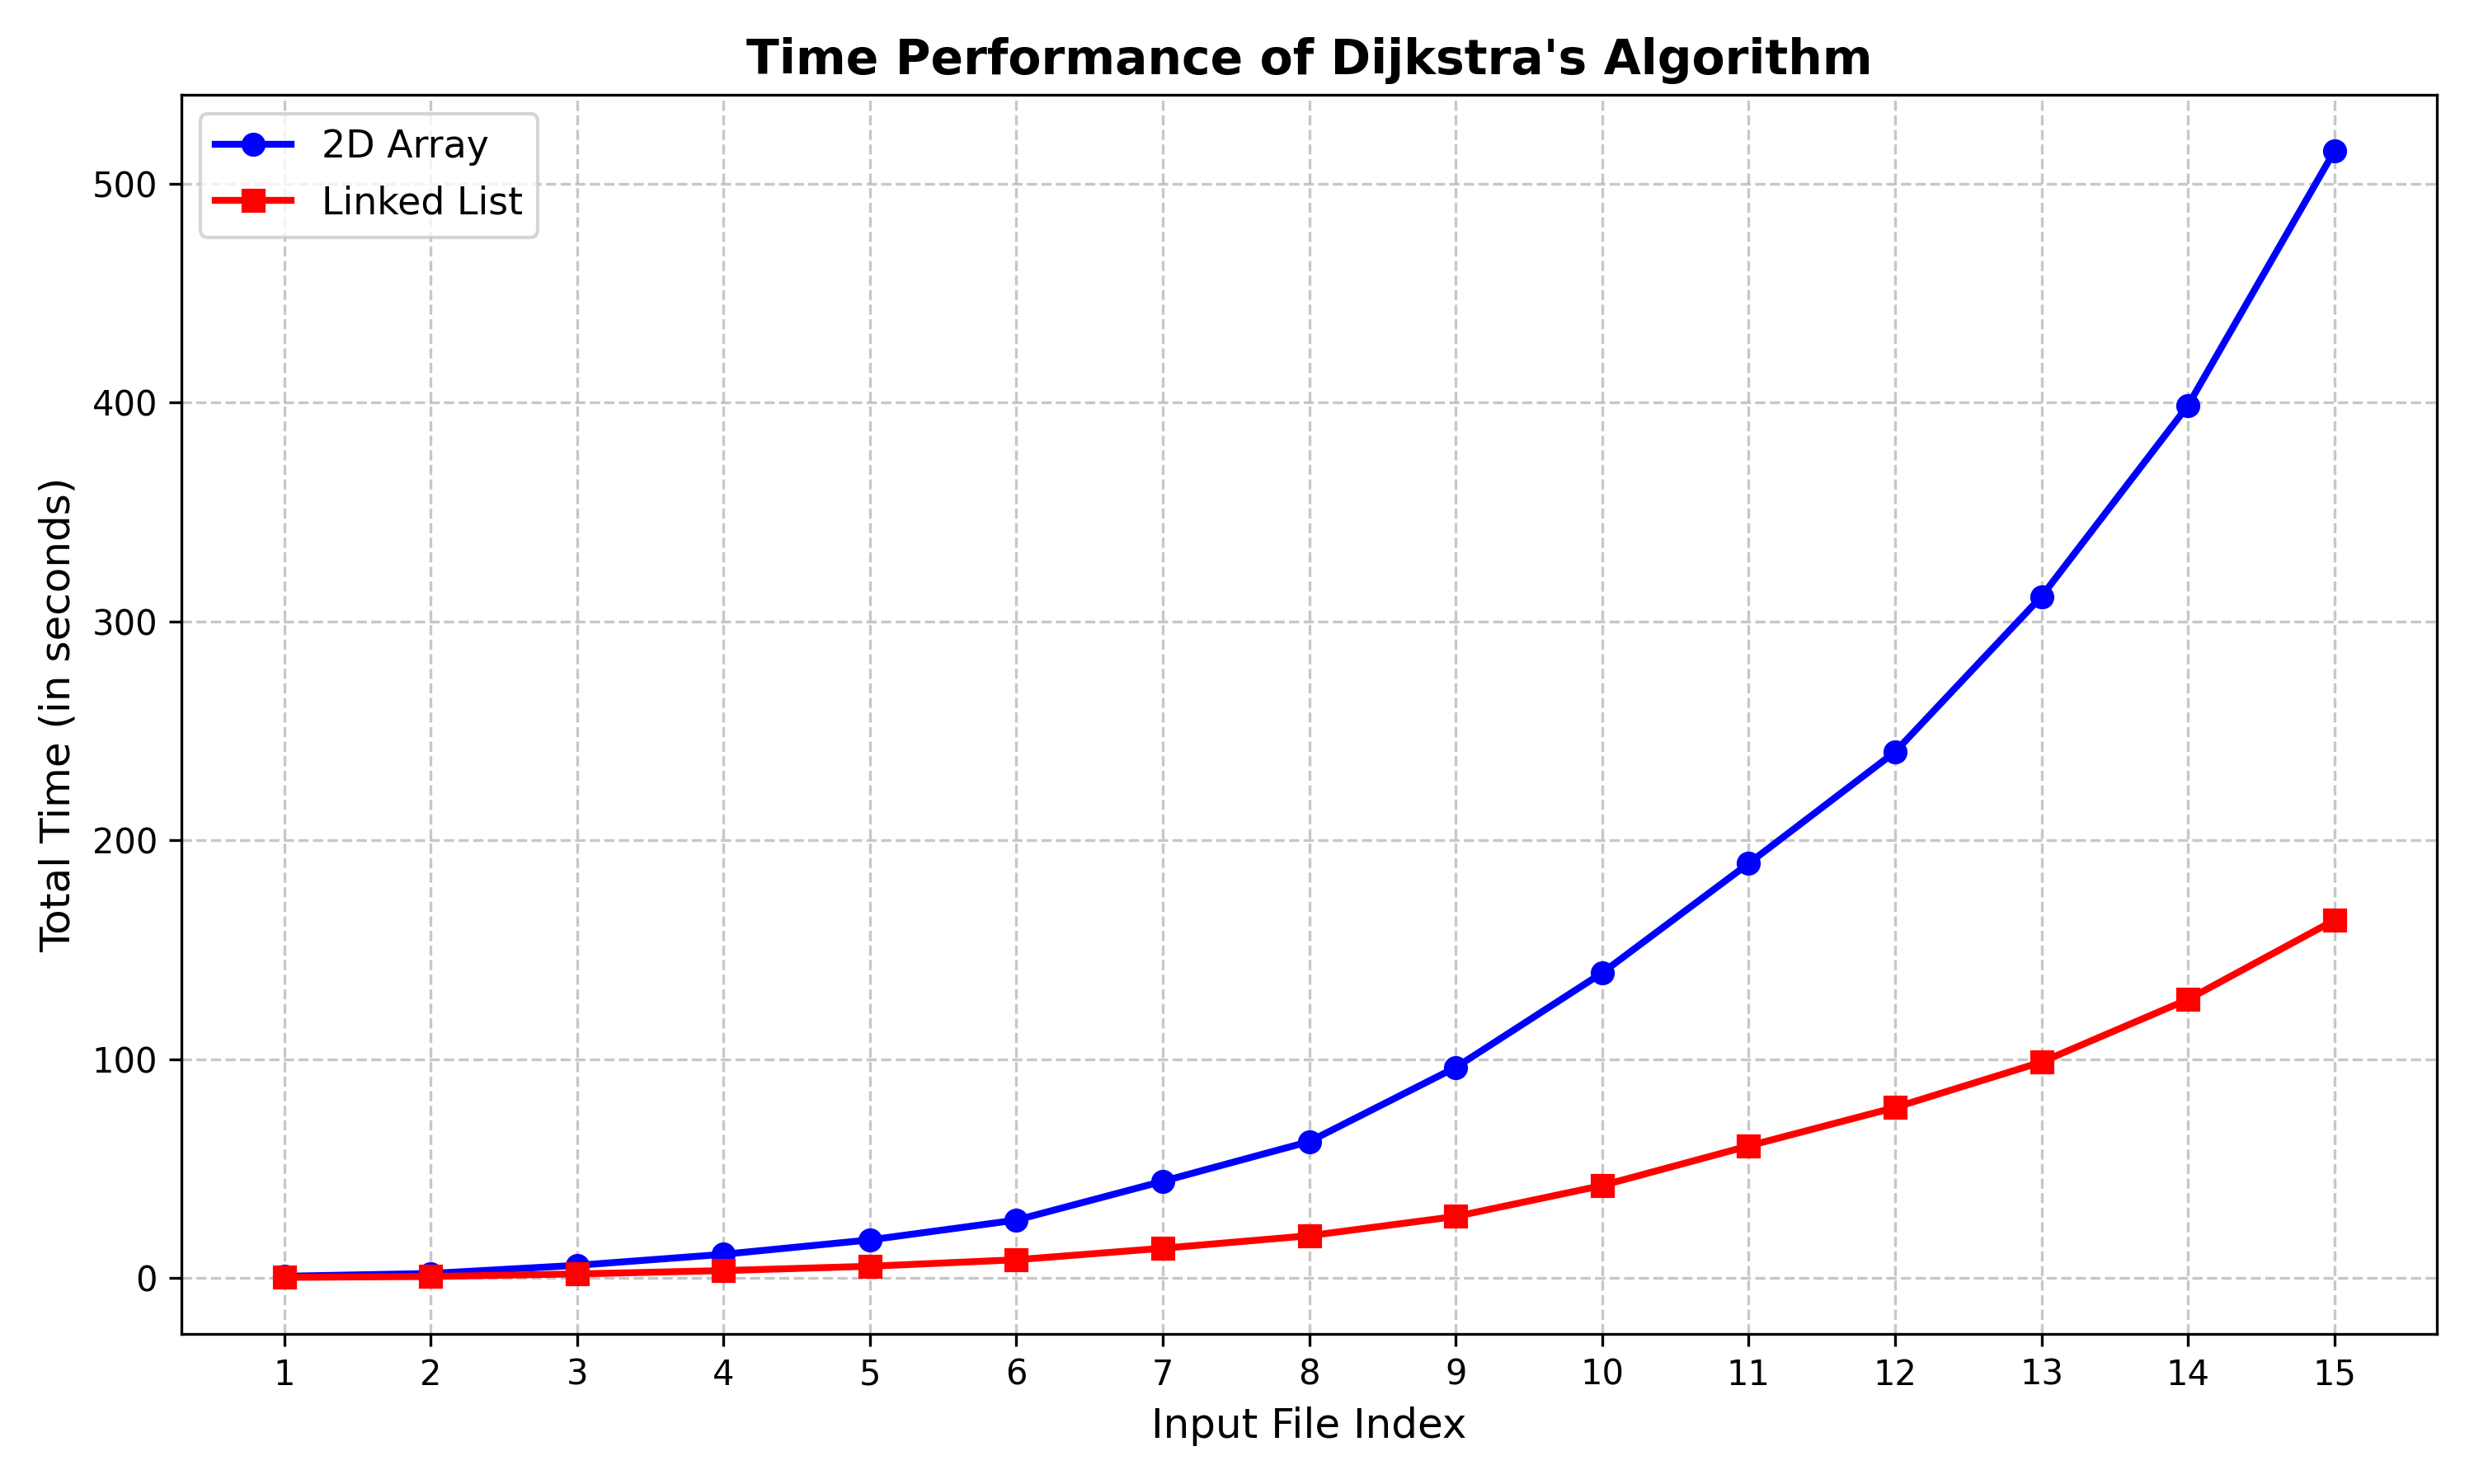
\includegraphics[width=0.7\textwidth]{Plot_Dijkstra_Time_Performance.png}
    \caption{Time Taken by Dijkstra's Algorithm for 2D Array and Linked List Implementations}
    \label{fig:dij_2d_time_performance}
\end{figure}
\subsection{Floyd's Algorithm}
\begin{figure}[H]
    \centering
    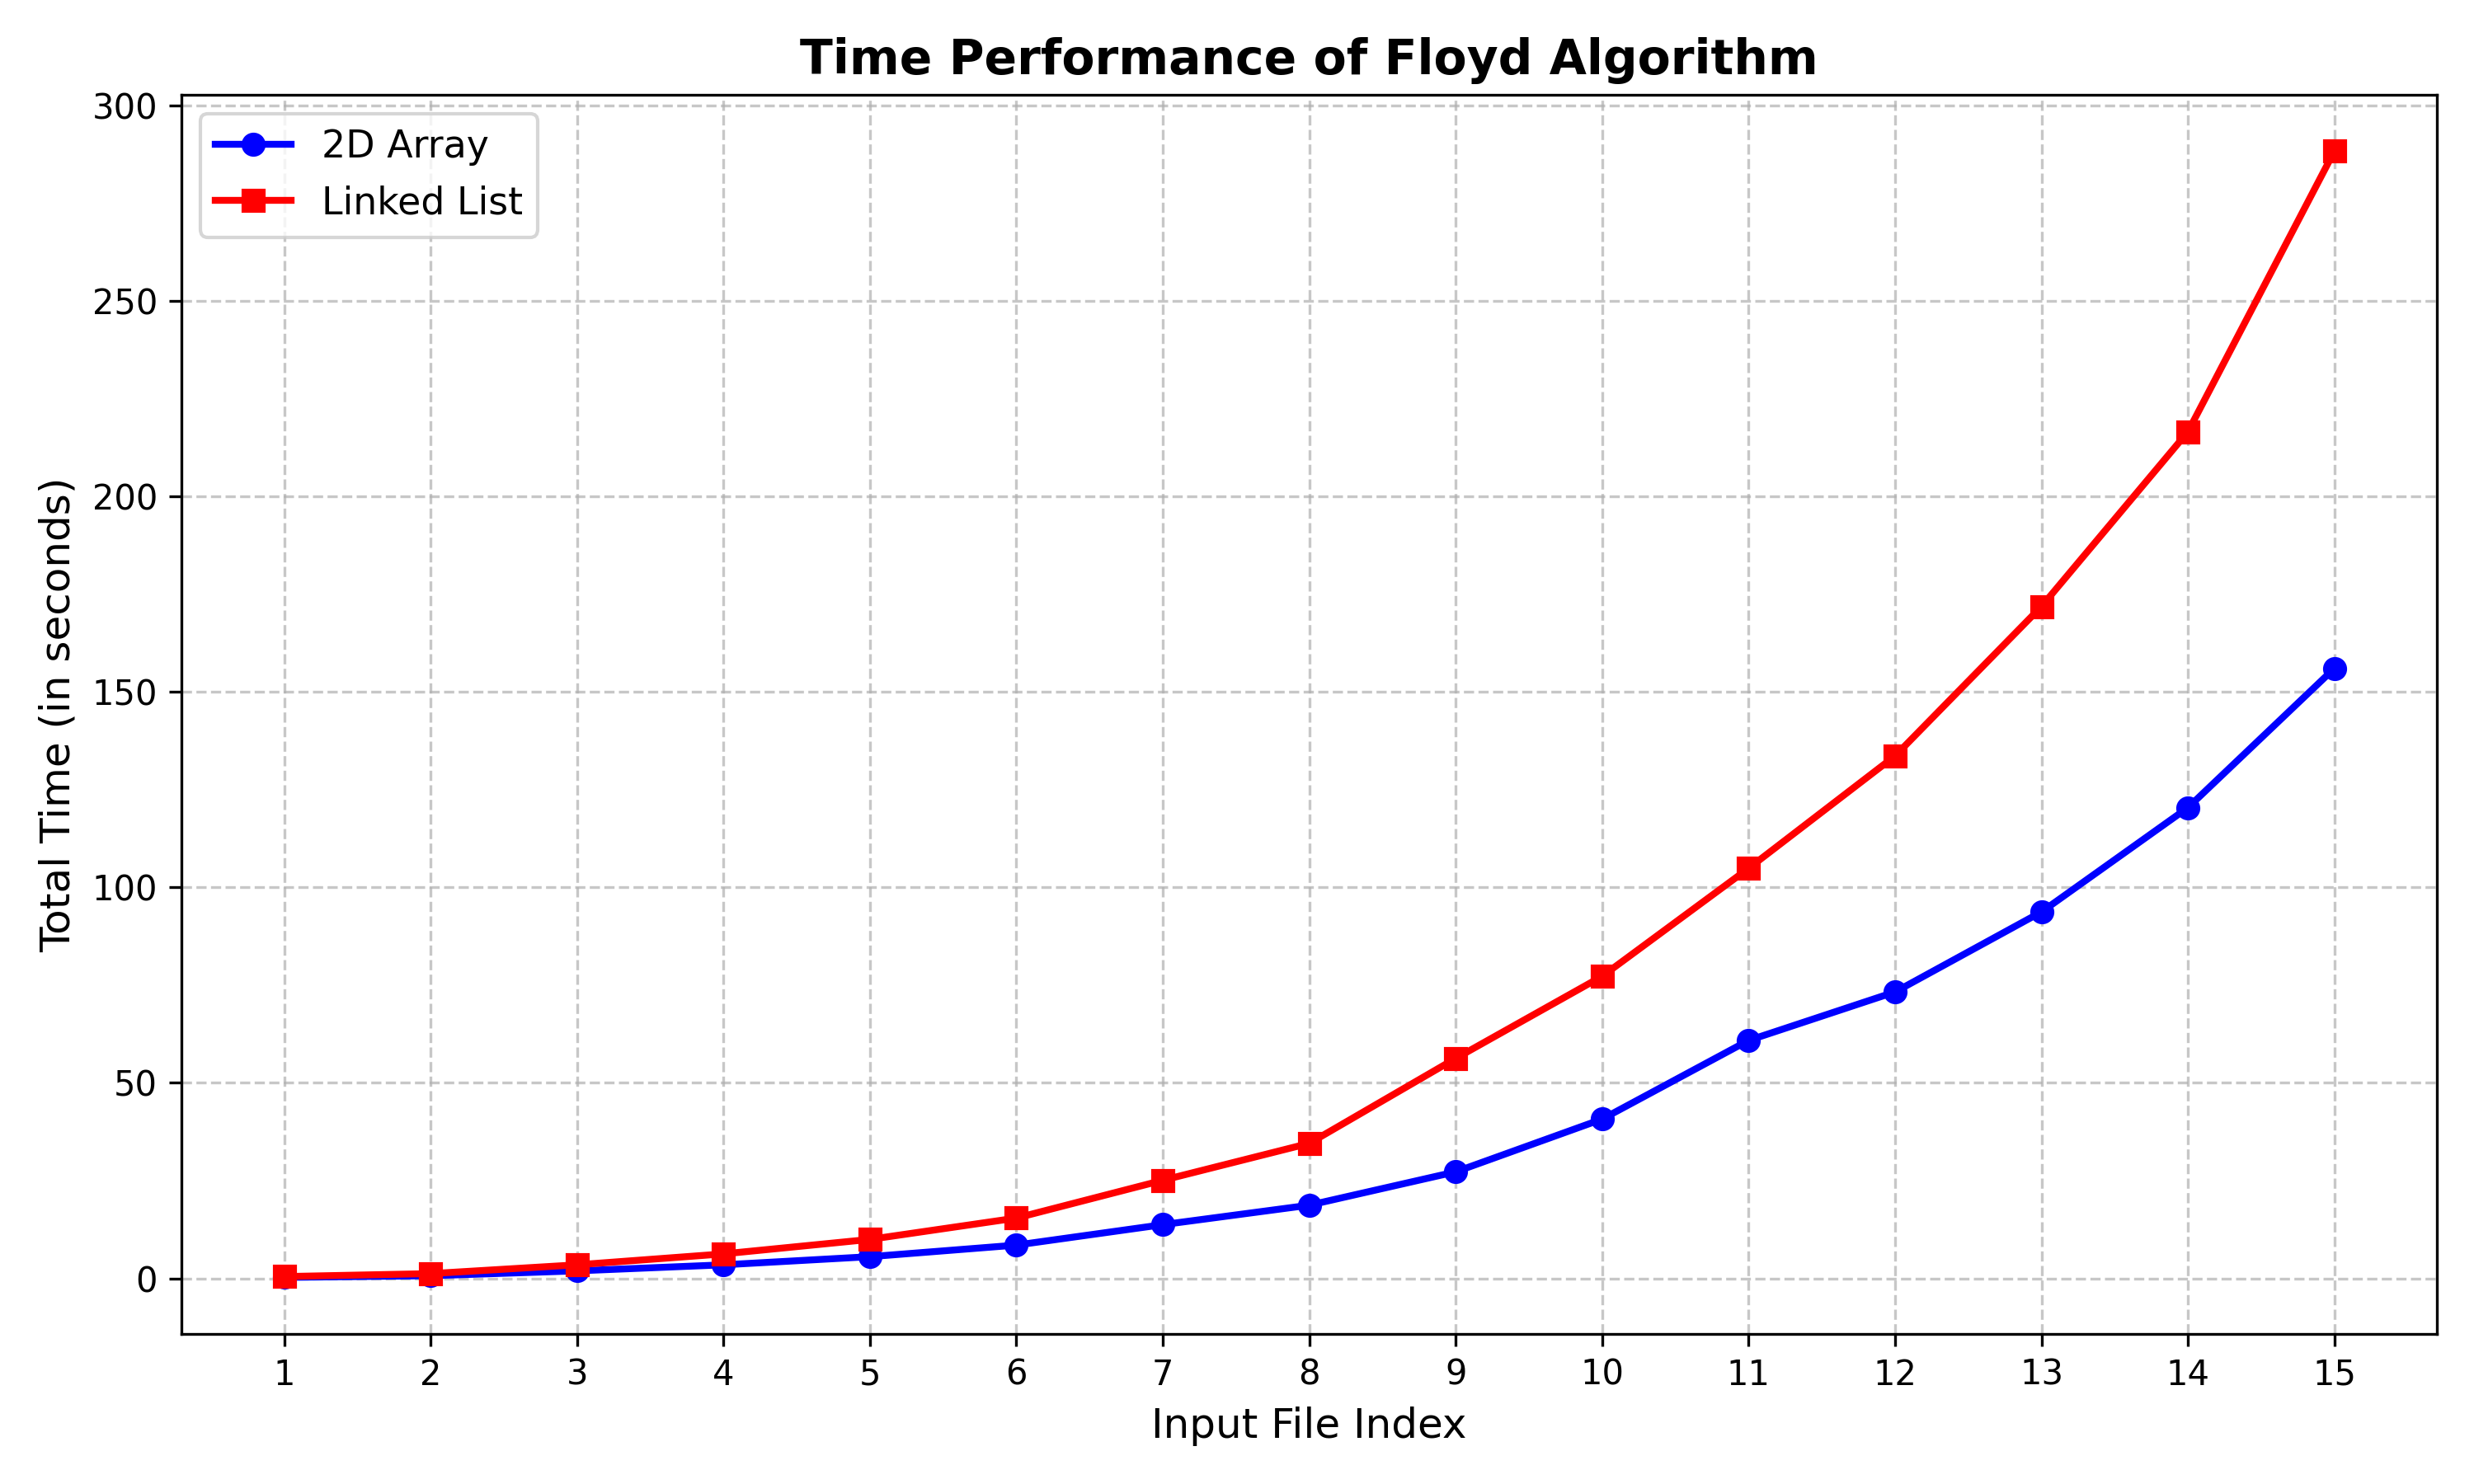
\includegraphics[width=0.7\textwidth]{Plot_Floyd_Time_Performance.png}
    \caption{Time Taken by Floyd's Algorithm for 2D Array and Linked List Implementations}
    \label{fig:floyd_2d_time_performance}
\end{figure}

\section{Time and Memory Usage}

Memory usage was computed based on the data structures used in each algorithm assuming
64-bit architecture. The tables below show the time taken and memory used by each algorithm
under both implementations.
\begin{table}[h!]
\centering
\renewcommand{\arraystretch}{1.2}
\begin{tabular}{|c|r|r|r|r|}
\hline
\textbf{File} & \textbf{Dijkstra (2D)} & \textbf{Dijkstra (LL)} & \textbf{Floyd (2D)} & \textbf{Floyd (LL)} \\
\hline
1 & 0.7235 & 0.2276 & 0.2435 & 0.4475 \\
2 & 2.0126 & 0.6304 & 0.6601 & 1.1999 \\
3 & 5.7263 & 1.7914 & 1.9083 & 3.4535 \\
4 & 10.7581 & 3.3236 & 3.4528 & 6.2476 \\
5 & 17.3465 & 5.3035 & 5.5380 & 9.9565 \\
6 & 26.4034 & 8.2791 & 8.4947 & 15.4086 \\
7 & 44.1399 & 13.5275 & 13.7268 & 25.0734 \\
8 & 62.2661 & 19.2583 & 18.7007 & 34.5197 \\
9 & 96.1438 & 28.0619 & 27.2312 & 56.2458 \\
10 & 139.3363 & 42.1884 & 40.7160 & 77.2402 \\
11 & 189.3239 & 60.2658 & 60.8352 & 104.8465 \\
12 & 240.3024 & 77.8398 & 73.2353 & 133.5842 \\
13 & 311.3177 & 98.6026 & 93.6975 & 171.8189 \\
14 & 398.5598 & 127.2308 & 120.3662 & 216.4860 \\
15 & 514.8188 & 163.3865 & 155.9801 & 288.2544 \\
\hline
\end{tabular}
\caption{Time Performance (in seconds) across all 15 input files}
\label{tab:time_perf}
\end{table}

\begin{table}[h!]
\centering
\renewcommand{\arraystretch}{1.2}
\begin{tabular}{|c|r|r|r|r|}
\hline
\textbf{File} & \textbf{Dijkstra (2D)} & \textbf{Dijkstra (LL)} & \textbf{Floyd (2D)} & \textbf{Floyd (LL)} \\
\hline
1 & 315.82 & 17.35 & 942.19 & 642.16 \\
2 & 621.55 & 24.34 & 1,857.23 & 1,257.84 \\
3 & 1,213.16 & 35.09 & 3,629.11 & 2,447.98 \\
4 & 1,807.97 & 43.73 & 5,411.25 & 3,643.27 \\
5 & 2,450.54 & 51.43 & 7,336.88 & 4,933.40 \\
6 & 3,281.12 & 59.72 & 9,826.31 & 6,599.85 \\
7 & 4,477.68 & 70.49 & 13,413.09 & 9,000.00 \\
8 & 5,592.35 & 79.13 & 16,754.77 & 11,234.95 \\
9 & 7,200.93 & 90.44 & 21,577.50 & 14,459.52 \\
10 & 9,454.19 & 103.19 & 28,333.59 & 18,974.01 \\
11 & 11,515.21 & 114.27 & 34,513.64 & 23,103.23 \\
12 & 13,655.06 & 125.53 & 40,930.36 & 27,390.51 \\
13 & 16,336.68 & 137.75 & 48,971.95 & 32,761.73 \\
14 & 19,209.52 & 150.15 & 57,587.25 & 38,515.63 \\
15 & 23,060.45 & 164.92 & 69,136.08 & 46,227.13 \\
\hline
\end{tabular}
\caption{Memory Usage (in KB) across all 15 input files}
\label{tab:mem_usage}
\end{table}
\newpage
The memory usage is calculated in the following way:
\begin{itemize}
  \item \textbf{Memory usage in Dijkstra's algorithm with 2D array:} \\
  Usage: adjacency matrix + distance array + previous array + visited array\\
  Formula: $(N^2 \times 8) + 2 \times (N \times 8) + N$ bytes \\

  \item \textbf{Memory usage in Dijkstra's algorithm with linked list:} \\
  Usage: Linked List size + distance array + previous array + visited array\\
  Formula: $(N \times 8) + (E \times 24) + 2 \times (N \times 8) + N$ bytes \\

  \item \textbf{Memory usage in Floyd's algorithm with 2D array:} \\
  Usage: 3x Matrices - Base, Dist, Next Node \\
  Formula: $3 \times (N^2 \times 8) + 3 \times (N \times 8)$ bytes \\

  \item \textbf{Memory usage in Floyd's algorithm with linked list:} \\
  Usage: Linked List size + 2x Matrices Dist, Next Node\\
  Formula: $(N \times 8) + (E \times 24) + 2 \times (N^2 \times 8) + 2 \times (N \times 8)$ bytes \\

\end{itemize}
where $N = nodes $ and $E = edges $. Total memory usage in each case:
\begin{itemize}
  \item \textbf{Dijkstra (2D):} $120,192.23 KB (~120.2 MB)$
  \item \textbf{Dijkstra (LL):} $1,267.53 KB (~1.27 MB)$
  \item \textbf{Floyd (2D):} $360,221.20 KB (~360.2 MB)$
  \item \textbf{Floyd (LL):} $241,191.21 KB (~241.2 MB)$
\end{itemize}
In terms of memory usage, Dijkstra's algorithm with linked list is significantly more efficient than the 2D array implementation, while Floyd's algorithm with linked list also uses less memory than the 2D array version, but both Floyd implementations use more memory than Dijkstra's.
\end{document}
